\subsection{UX Diagrams}

The RASD already presented the main mobile interfaces for generic users and third parties, in this section the relations among them is shown in detail. UX diagrams below explain which forms have to be completed in which screen, and what flow is followed by the latters. Obviously, only mobile interfaces are dealt with: the script flow is the same as the third parties' UX Diagram.

\bigskip
The two UX Diagrams below are one for the generic user experience and the other for the third party experience.
\bigskip

\begin{center}
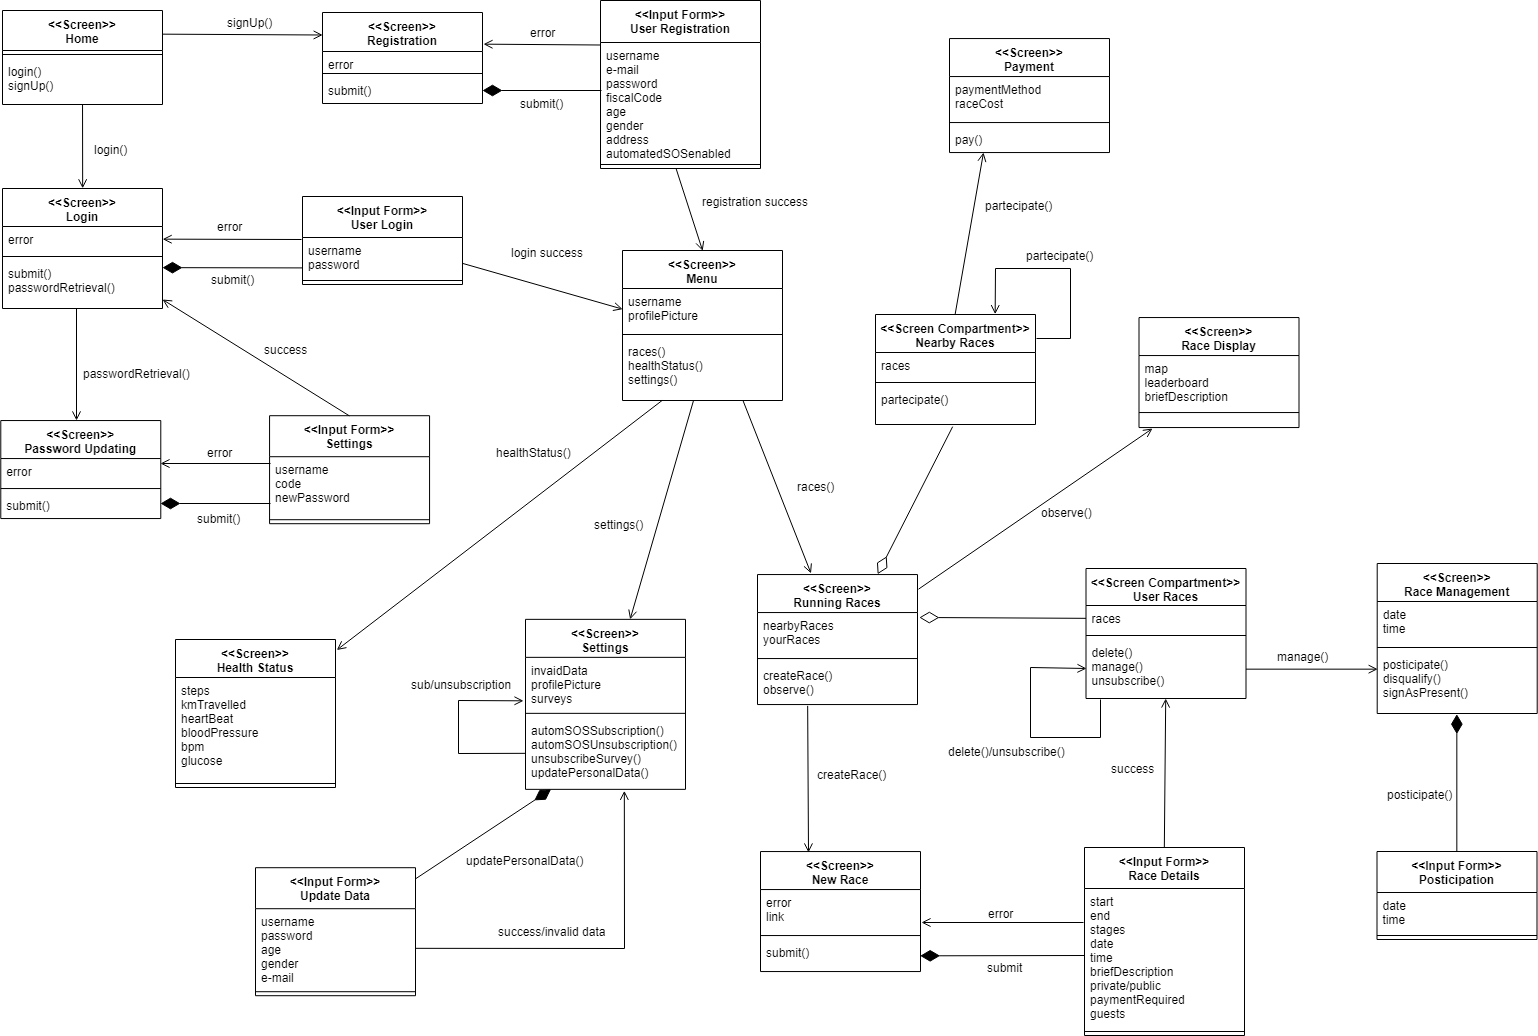
\includegraphics[scale=0.3]{sections/diagrams/UX}
\newline
\captionof{figure}{UX Diagram of a the Mobile Application-generic user}
\end{center}

As regards the race partecipation, the two "partecipate()" refers to the partecipation when a payment is required and when it doesn't. So, according to the race organization payment request, "partecipate()" will lead only to one screen, exclusively.

\begin{center}
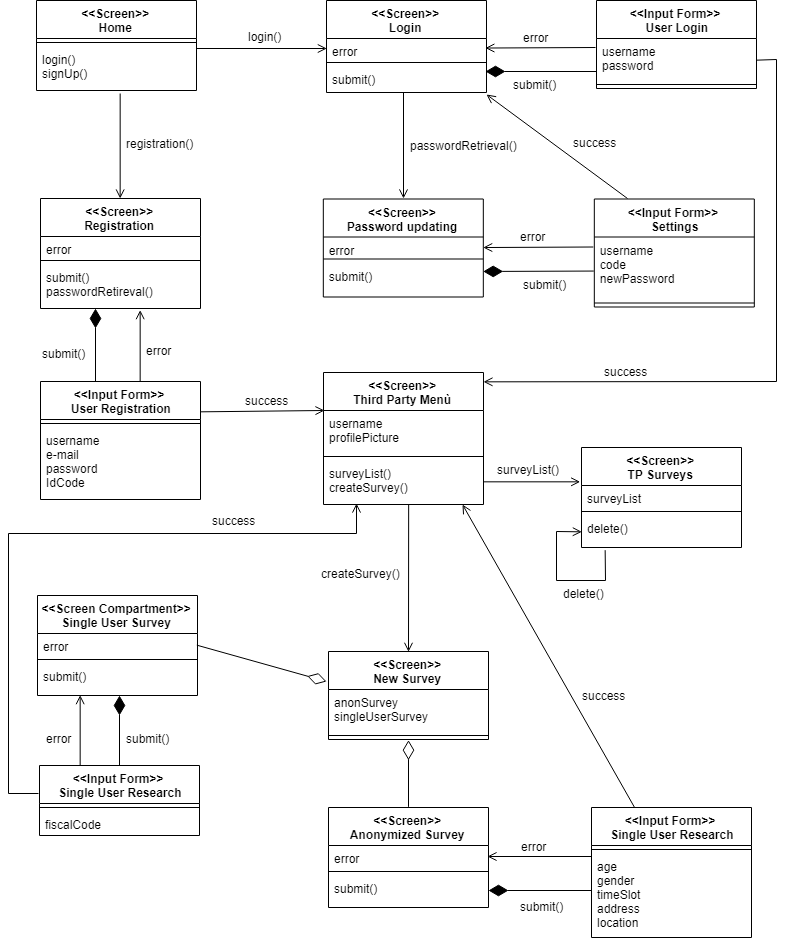
\includegraphics[scale=0.5]{sections/diagrams/thirdPartyUX}
\newline
\captionof{figure}{UX Diagram of a the Mobile Application-third party}
\end{center}